\section{Routing in Wired/Wireless Internetworks with OSPF}
\label{s:wospf}
%
Protocols reviewed in section \ref{s:specific} have been specifically designed for spontaneous wireless networks. However, the increasing deployment of wireless technologies and the integration of different sorts of flexible networks with the Internet is leading to more complex inter-networks, neither purely wired networks nor purely spontaneous wireless networks, resulting from the interconnection of wireless mesh networks with fixed, wired networking infrastructure, inside Internet's Autonomous Systems. Figure \ref{f:cpd_as} shows schematically a {\em compound Autonomous System}, in which fixed and wireless mesh networks are interconnected in the same routing domain. \ \\ \ \\
%
\begin{figure}[h]
\centering
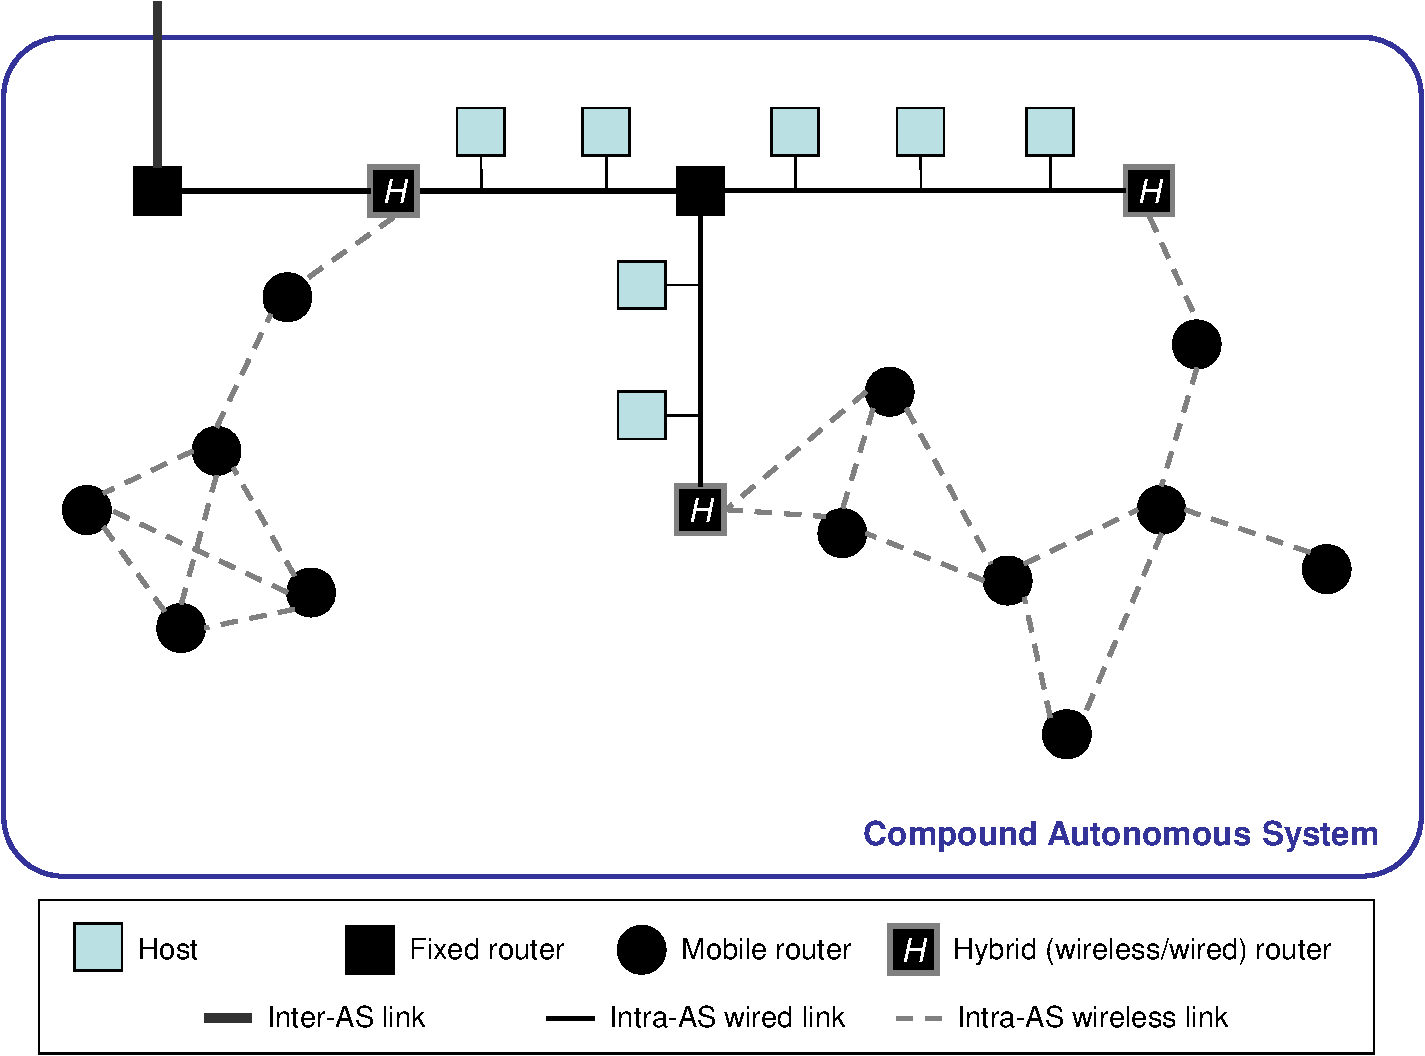
\includegraphics[width=0.8\textwidth]{Figures/cpd_as-crop.pdf}
\caption{A compound Autonomous System.}
\label{f:cpd_as}
\end{figure}
%
In these scenarios, a classic IGP (in IP networks, typically OSPF) is used for routing in the fixed network inside the AS. Rather than using an additional protocol for routing in the wireless mesh network inside the AS, it makes sense to explore approaches {\em extending} the protocol already used in the AS, so that it can take into consideration the issues described in section \ref{s:comm_wless}, run efficiently over wireless dynamic networks, handle the heterogeneity of the hybrid internetwork and thus perform routing over the whole compound AS. Extension for hybrid internetworks of a protocol already in use can significantly reduce the transition costs (technical implementation, engineer training...), as only minor changes, or no changes at all, will be needed in the networks using the original protocol. It may be also benefial in terms of networking management complexity and routing performance, as a single (extended) routing protocol is more bearable than several protocols running in different parts of the internetwork. In the latter case, route distribution between different protocols operating at wireless and wired networks needs to be performed in specific {\em hybrid routers} (see Figure \ref{f:cpd_as}); this adds another layer of networking complexity and is likely to cause routing suboptimality. The advantages of extending a protocol in use come, however, at the expense of increasing the complexity and narrowing the space for optimization in the extended protocol, which needs to cope efficiently with a broader range of networking scenarios.\ \\ \ \\
%
This section reviews the IETF extensions of the Open Shortest Path First (OSPF) protocol for MANETs. Section \ref{ss:ospf} shortly reviews the basics of OSPF, the main IGP for IP networks and a major representative of the link-state routing family, and indicates the reasons that prevent OSPF to be used ``as-is'' in wireless multi-hop ad hoc networks. Section \ref{ss:ospfmanet} describes the main elements of the three extensions for MANETs standardized by the IETF: Multi-Point Relays (MPR-OSPF, specified in RFC 5449), MANET Designated Routers (OSPF-MDR, specified in RFC 5614) and Overlapping Relays (OR/SP, specified in RFC 5820).
%
\subsection{Open Shortest Path First Protocol (OSPF)}
\label{ss:ospf}
%
OSPF \cite{rfc2328,rfc5340} is a link-state routing protocol for IP networks. Each router maintains a local {\bf Link State Database} (LSDB), representing the full network topology. The protocol ensures that each router has the same LSDB and, thus, the exact same view of the network topology. Paths to every possible destination are derived from the {\bf Shortest Path Tree} (SPT) that every router computes, by way of Dijkstra's algorithm \cite{dijkstra59}. \ \\ \ \\
%
Routers acquire information about their 2-hop (bi-directional) neighborhood and advertise their own presence and their 1-hop neighbors by periodically exchanging {\bf Hello} messages with all their neighbors, in the way described in section \ref{ss:nd}. \ \\ \ \\
%
Topology information is also disseminated through the network by way of {\bf Link State Advertisements} (LSAs). Each such LSA lists mainly the current adjacencies of the router which generated the LSA. The local LSDB stored by a router contains the most recent LSAs received from every other router in the network. \ \\ \ \\
%
Each router synchronizes its LSDB with a subset of its bidirectional neighbors. Synchronization between two neighboring routers is performed on a master-slave basis, by exchanging summaries of all LSAs in their LSDB, and then allowing each router to request retransmission of missing or locally outdated link-state advertisements. Links between a router and its synchronized neighbors are called {\bf adjacencies}. The set of adjancencies is expected to form a network-wide connected backbone, connecting all routers in the network, in order to ensure paths can be computed correctly.\ \\ \ \\
%
Finally, routers also acquire remote topology information by receiving LSAs. LSAs are flooded through the entire network in reliable fashion (explicit acknowledgements and retransmissions) via the backbone formed by adjacencies. Thus, any router which has formed adjacencies must advertise this periodically by way of constructing an LSA and performing LSA flooding.
%
\begin{equation}
\textrm{SPT links} \subset \textrm{Adjacent links} \subset \textrm{Bi-directional links}
\end{equation}
%
Remote topology information is then used for the construction of the Shortest Path Tree: each router computes the shortest paths based on the information contained in the set of received LSAs. \ \\ \ \\
%
This operation implies that OSPF exchanges control traffic and performs routing according to two principles:
%
\begin{enumerate}
\item Data traffic is routed to the corresponding destination through links contained in the Shortest Path Tree.
\item Data and control and traffic (LSAs and acknowledgements) is sent over adjacent (synchronized) links.
\end{enumerate}
%
\paragraph{Interface Types} 
%
Rules for flooding and adjacency handling vary for the different \emph{interface types} supported by OSPF. Four main interface types are specified in RFC 2328 \cite{rfc2328}:
%
\begin{itemize}
\item \emph{Point-to-point interfaces} are those connected to point-to-point links. Such a link only permits communicating with a single (neighboring) interface.
\item \emph{Broadcast interfaces} participate in a broadcast link, in which any interface can directly communicate with any other interface. A classic example of broadcast link is Ethernet.
\item \emph{Non-Broadcast Multiple Access (NBMA) interfaces}, for non-broadcast networks ({\em i.e.}, networks supporting more than two routers, but without broadcast capability) in which each pair of interfaces can communicate directly. This interface type may be used with X.25 and ATM networks with Switched Virtual Circuits (SVC).
\item \emph{Point-to-multipoint interfaces}, for those non-broadcast networks in which direct communication between any pair of interface is not guaranteed. This may be the case, for instance, in Frame Relay networks using only Permanent Virtual Circuits (PVC), if not every pair of routers have a PVC between them. 
\end{itemize}
%
OSPF only provides support for the two first interface types. In the NBMA and point-to-multipoint cases, OSPF {\em emulates} the behavior of a broadcast link and point-to-point links, repectively. For NBMA networks, LSA flooding and LSDB synchronization are handled by way of {\bf Designated Routers} (DRs). A Designated Router (as well as a Backup Designated Router, BDR, expected to become DR in case of DR's failure) is elected from among routers whose interfaces are connected to the same link. DRs (and BDRs) form adjacencies with all the routers connected to the same link, and the Designated Router becomes responsible for flooding of LSAs, originated by routers on that link. A router point-to-multipoint link, in turn, is handled as a set of independent point-to-point links, one per neighboring router with which direct communication is available.
%
\subsection{MANET Extensions: A Wireless Interface for OSPF}
\label{ss:ospfmanet}
%
Standard interface types for non-broadcast networks (point-to-multipoint and NBMA) are not adapted for operation in a wireless multi-hop ad hoc network. As discussed in section \ref{ss:issues}, routers in a wireless multi-hop network may not agree on which routers are connected to a given link. This implies that the DR-based mechanisms of NBMA cannot be directly used in wireless multi-hop ad hoc networks. DR election may be inconsistent between different routers, causing flooding to disfunction and, possibly even preventing the protocol from converging. The use of the point-to-point interface, in turn, does not scale in these dynamic networks: point-to-point emulation for every pair of interfaces directly reachable to each other causes an excessive control traffic overhead, even for relatively small networks, as shown experimentally in Henderson {\em et al.} \cite{henderson03}. This fact has led the research and industrial OSPF community to develop a new interface type to support the characteristics of wireless multi-hop ad hoc networks.\ \\ \ \\
%
This new interface type needs to optimize the operation of (1) describing local topology in LSAs, (2) performing LSA flooding and (3) establishing and maintaining adjacencies in the context of wireless communication. Different approaches have been explored at the IETF, which have led to three different extensions of OSPF, consisting of three different interfaces for wireless multi-hop networks (or MANETs, in IETF's terminology).
%
\paragraph{Multi-Point Relays} MPR-OSPF \cite{rfc5449} use Multi-Point Relays (MPR \cite{mpr-hicss2002}, see section \ref{ss:flood}) to optimize topology description, LSA flooding and LSDB synchronization. Nodes select MPRs from among their bidirectional neighbors in order to provide 2-hop coverage, and use them to disseminate their LSAs. A router becomes adjacent to both neighbors which it has selected as multi-point relays (MPRs) and neighbors which have selected the router as their multi-point relay (MPR selectors). Each router advertises in its LSAs its own MPRs and MPR selectors; consequently, the Shortest Path Tree is constructed over the set of adjacencies. 
%
\paragraph{Overlapping Relays \& Smart Peering} The Overlapping Relays / Smart Peering (OR/SP) extension of OSPF \cite{rfc5820} floods LSAs via MPR as in MPR-OSPF, where the multi-point relays selected among the adjacent (synchronized) neighbors of the electing router. Adjacencies are selected following the Smart Peering (SP) rule, in which a neighbor becomes adjacent if it is not already reachable through the computing router's current Shortest Path Tree. The SP criterion reduces dramatically the number of synchronized links in the network. LSAs list adjacent neighbors, and may also list additional bidirectional neighbors (so-called \emph{unsynchronized adjacencies}). The SPT is thus constructed over adjacencies and a subset of bidirectional neighbors. 
%
\paragraph{MANET Designated Routers} OSPF-MDR \cite{rfc5614} relies on two Connected Dominating Sets (CDS): the MANET Designated Routers (MDR) backbone and the Backup MDRs (BMDR) backbone. Both extend the standard OSPF (for NBMA networks) notions of ``Designated Routers" and ``Backup Designated Routers" to MANETs. This implies that routers behave differently depending on their role. MDRs are the only nodes allowed to flood LSAs. Every non-MDR router becomes adjacent at least to the closest MDR, and MDRs must become adjacent to other MDRs. LSAs list a configurable subset of links of the originator, which must at least include the adjacent neighbors. The SPT is thus constructed over adjacencies and a subset of bidirectional neighbors. \ \\ \ \\
%
Compatibility with the OSPF routing philosophy detailed in section \ref{ss:ospf} varies significantly depending on the considered OSPF extension. MPR-OSPF is designed to preserve the two principles in OSPF routing: shortest, synchronized paths for data traffic and synchronized links for control traffic. Under the Overlapping Relays extension, data traffic paths are synchronized, but they are not necessarily optimal, as routers only synchronize a small fraction of their available links. Although providing several configuration parameters to tune the protocol's performance, the MANET Designated Routers (OSPF-MDR) also try to minimize the control traffic by reducing the number of synchronized links, even when this may lead to path suboptimality for data traffic.
%
\paragraph{Preserving OSPF routing principles} Performed experiments suggest that extensions providing (theoretical) shortest paths for data traffic achieve a better performance than those neglecting shortest paths or allowing suboptimal routing in a wireless multi-hop network \cite{aircc, porto}. Further analysis showed that preserving the second principle (all traffic is sent over synchronized links) in OSPF over mobile ad hoc networks, in the way that MPR-OSPF does, requires a significant amount of overhead due to the LSDB exchange between routers becoming {\em adjacent} (synchronized), and does not bring substantial benefit, due to short lifetime of several synchronized links in a wireless multi-hop dynamic network \cite{hicss2011}.
%
\paragraph{Why maintain LSDB synchronization in Extended OSPF ?} LSDB synchronization between two routers proves useful in classic (wired) Internet internetworks, but is an expensive operation to perform in a dynamic (wireless multi-hop or mobile ad hoc) network. This is the reason why other link-state protocols such as OLSR, designed specifically for wireless mesh and mobile ad hoc networks, does not provide any mechanism for synchronizing the LSDBs of neighboring routers: topology information is only disseminated through the network by way of LSA flooding (see section \ref{sec:olsr}). In the case of extended OSPF, there are two reasons for maintaining the notion of LSDB synchronization: 
%
\begin{enumerate}
\item {\bf OSPF backwards compatibility}. In standard OSPF \cite{rfc2328,rfc5340}, the notion of {\em adjacency} is essential in the protocol's architecture and the router's operation, regardless of the specific types used for running OSPF in the router's interfaces.
\item {\bf Routing in heterogeneous internetworks}. Unlike OLSR, extended OSPF is expected to run over hybrid internetworks (or compound Autonomous Systems, see Figure \ref{f:cpd_as}), that is, internetworks in which wired networks handled by standard OSPF interface types coexist and are interconnected with wireless multi-hop networks using the adapted wireless interface of (extended) OSPF. In these scenarios, in which some nodes (with wireless interfaces) are exposed to frequent disconnections from the network (meaning that their LSDBs may be no longer updated for a while) and others maintain stable links with their neighbors (those with wired interfaces), the fact that every router is expected to synchronize its LSDB with {\em at least} one of its neighbors provides an upper bound for the maximum time that a router $A$ (in the wireless region of the internetwork) stays {\em disconnected} (that is, unaware of its local topology) from another router $B$ (in the wired region of the internetwork) after missing an LSA flooded by router $B$. This becomes an issue as the time between consecutive LSA flooding processes from $B$ is typically high -- as wired links are stable and thus require less frequent updates about their state than wireless ones.
\end{enumerate}
%
\paragraph{Further Extensions: adapted LSDB synchronization, MPR+SP and SLOT-OSPF} In this context, some additional approaches can be explored beyond the three standardized extensions of OSPF. Clausen {\em et al.} \cite{secon2004}, for example, propose a LSDB synchronization process based on the periodic broadcasting of {\em signatures} of the LSDB by every router to its neighborhood. These signatures allow neighbors of the originator to detect topology inconsistencies with its own LSDB, and request unicast retransmission of the corresponding LSAs. This turns the standard OSPF synchronization mechanism, based on a router-to-router LSDB exchange, to a router-to-neighborhood mechanism that takes advantage from the semibroadcast nature of communication in a wireless multi-hop network.

Without modifying the standard OSPF adjacency-forming process, LSDB synchronization can be kept, but the number of adjacencies per router should be reduced as much as possible, given the high cost of synchronization in terms of overhead and its small benefit in a dynamic network, with short-lived links. Data traffic should be sent over shortest paths (that is, optimal paths over the network, according to the available LSDB information and the metric in use), but these paths do not need to be synchronized. This leads to combine in the same OSPF extension the mechanisms to provide shortest paths (MPR selection for topology description) and the mechanisms reducing the most the number of adjacencies to be established per router ({\em e.g.}, the Smart Peering rule used in the Overlapping Relays extension). The resulting extension, denominated MPR+SP, presents a better routing performance than extensions MPR-OSPF and OR/SP in which it is based, as shown in Cordero {\em et al.} \cite{hicss2011}. Similarly, extension SLOT-OSPF \cite{mass2010} using the Relative Neighbor Graph (RNG \cite{toussaint80}) for establishing adjacencies and MPR selection for computing shortest paths, also achieves better results in terms of delivery ratio and control traffic overhead than the standard extension to which it compares. In both cases (MPR+SP and SLOT-OSPF) shortest path computation, for which a comprehensive view of the network topology (with most of the links) is required, is splitted from the adjacency-forming criterion, which aims to reduce as much as possible the number of LSDB synchronizations to be performed. This split enables a further optimization of the protocol routing performance.

